\title{Warm-Up for April 15th, 2022}
\author{Dr. Jordan Hanson - Whittier College Dept. of Physics and Astronomy}
\date{\today}
\documentclass[12pt]{article}
\usepackage[a4paper, total={18cm, 27cm}]{geometry}
\usepackage{graphicx}
\usepackage{amsmath}
\usepackage{subcaption}
\usepackage{bm}
\def\rcurs{{\mbox{$\resizebox{.16in}{.08in}{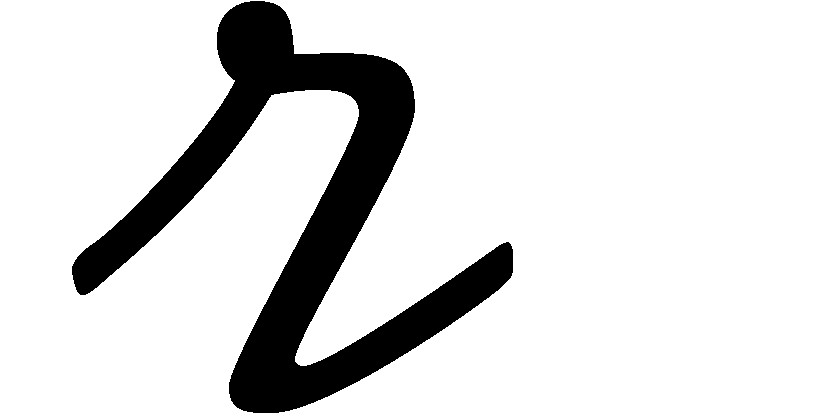
\includegraphics{ScriptR}}$}}}
\def\brcurs{{\mbox{$\resizebox{.16in}{.08in}{
\includegraphics{BoldR}}$}}}
\def\hrcurs{{\mbox{$\hat \brcurs$}}}
 
\begin{document}
\maketitle
\small
\section{Memory Bank}
\begin{enumerate}
\item Magnetic boundary conditions:
\begin{align}
B_{\perp}^{above} &= B_{\perp}^{below} \label{eq:1} \\
B_{||}^{above} - B_{||}^{below} &= \mu_0 K \label{eq:2} \\
\mathbf{B}_{above} - \mathbf{B}_{below} &= \mu_0 \left(\mathbf{K} \times \hat{\mathbf{n}}\right) \label{eq:3} \\
\mathbf{A}_{above} &= \mathbf{A}_{below} \\
\frac{\partial\mathbf{A}_{above}}{\partial n} - \frac{\partial\mathbf{A}_{below}}{\partial n} &= -\mu_0 \mathbf{K} \\
\end{align}
\end{enumerate}

\begin{figure}[ht]
\centering
\begin{subfigure}{0.3\textwidth}
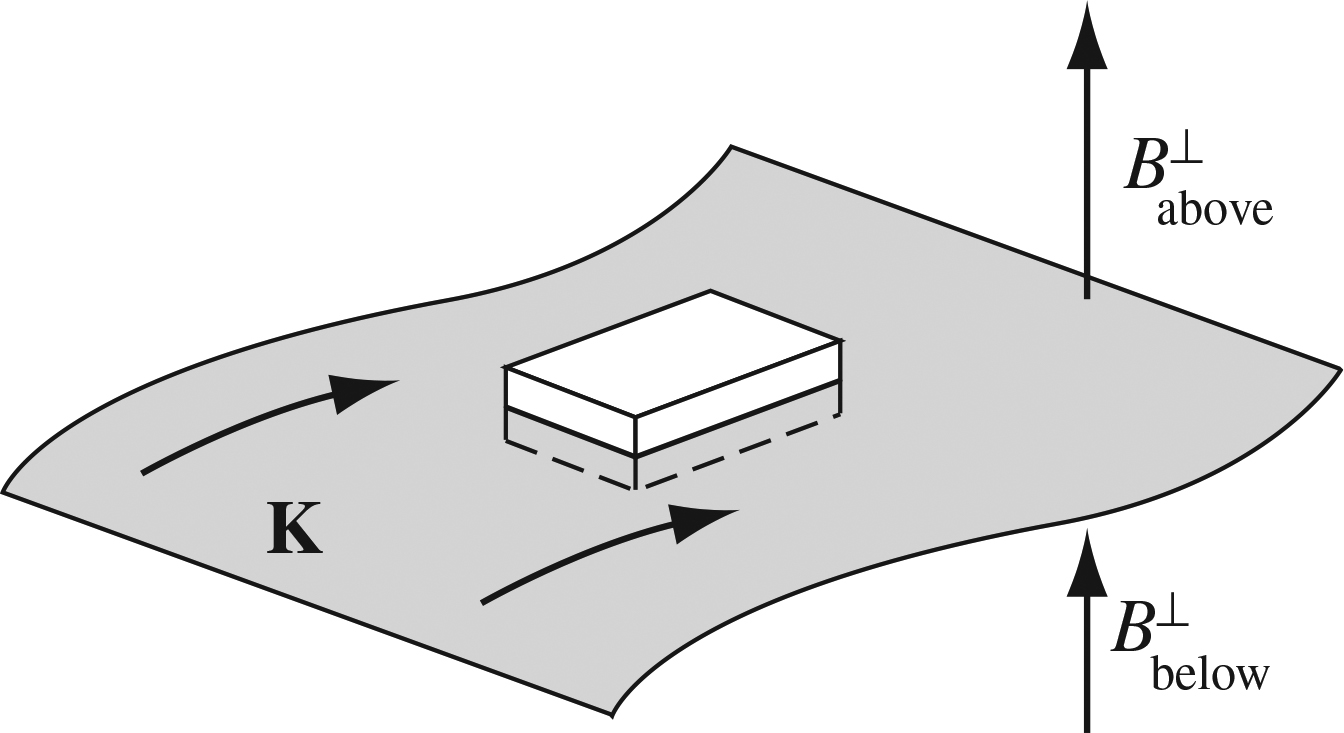
\includegraphics[width=\textwidth]{figures/5_49.jpg}
\caption{ }
\end{subfigure}
\hspace{0.5cm}
\begin{subfigure}{0.3\textwidth}
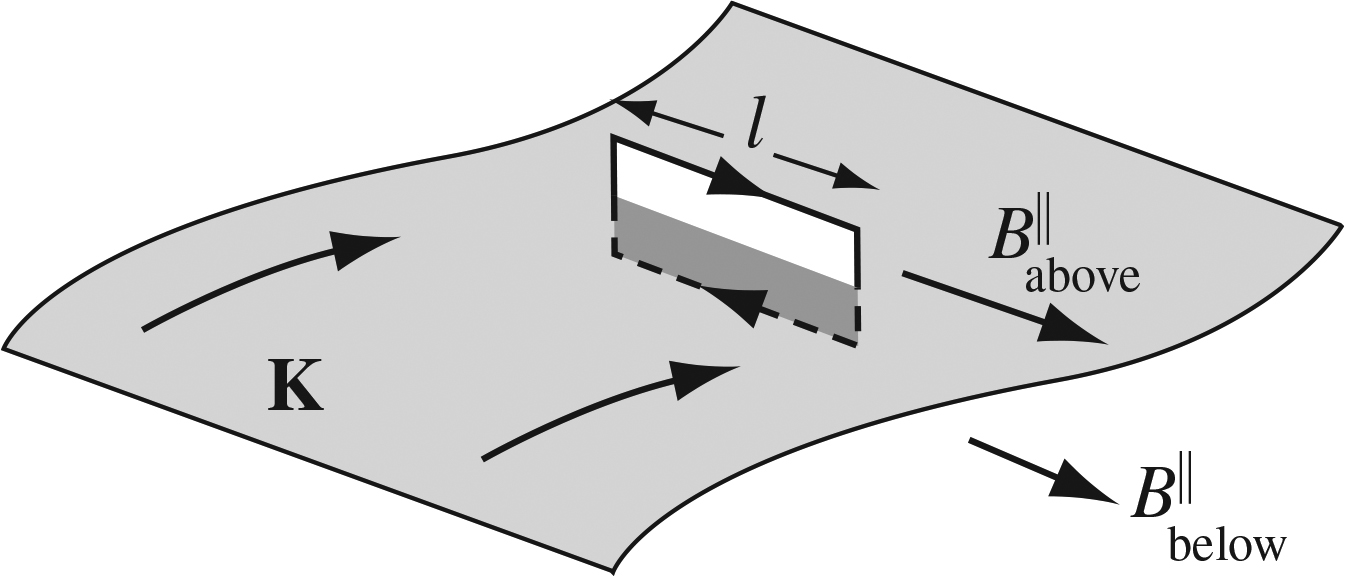
\includegraphics[width=\textwidth]{figures/5_50.jpg}
\caption{ }
\end{subfigure}
\caption{\label{fig:1} (a) Boundary conditions for $\mathbf{B}$-fields, perpendicular to the surface. (b) Boundary conditions for $\mathbf{B}$-fields, parallel to the surface.}
\end{figure}

\section{Magnetic Boundary Conditions}

\begin{enumerate}
\item Picture a long solenoid with current $I$ and turns per unit length $n$.  Derive the internal $\mathbf{B}$ and $\mathbf{A}$-fields, and check each boundary condition above.
\end{enumerate}
\end{document}